\chapter{System architecture}
\label{ch:architecture}

\lhead{Chapter 5. \emph{System architecture}}

This chapter describes the system architecure in detail.
We follow a top-down approach, giving an overview of the architecture and then detailing each part in a separate section.

\section{Overview}

The product consists of multiple, interoperable systems including:
\begin{enumerate}[1.]
	\item an integration platform (\textit{NIPEN})
	\item a front-end to the integration platform
	\item two Android applications
	\item a web service
\end{enumerate}

Figure \ref{figure:architecture} shows the overall system architecture.
In the following sections we provide a detailed description of the each part of the system.

\begin{figure}[h]
\centering
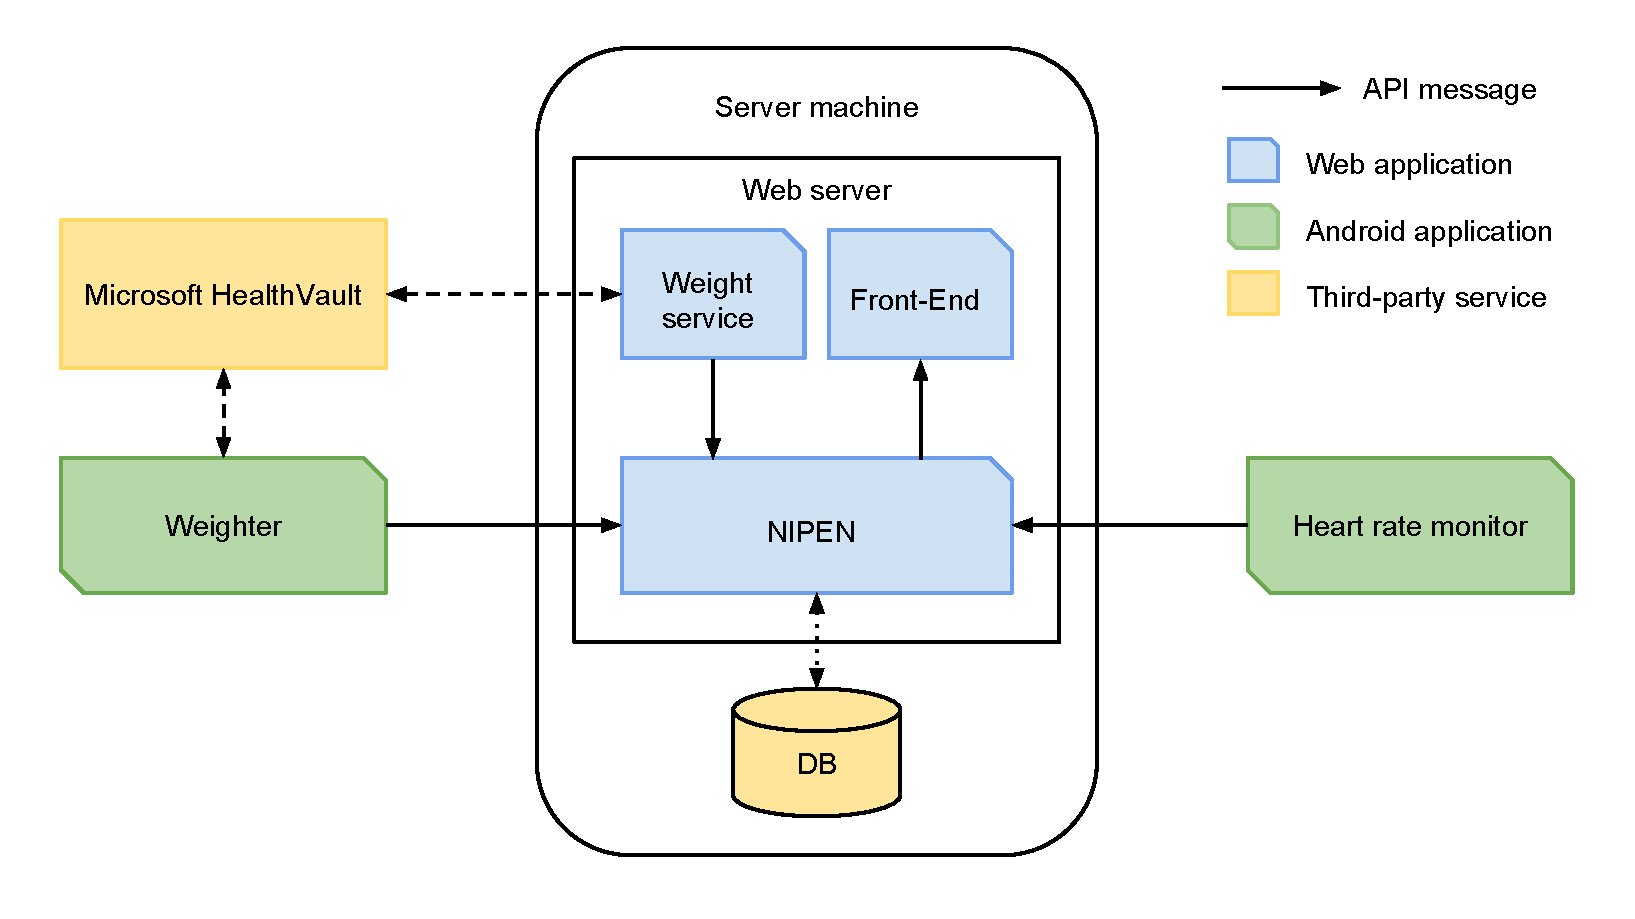
\includegraphics[scale=0.5]{../Figures/architecture.pdf}
\caption{System architecture}
\label{figure:architecture}
\end{figure}

\section{Architectural drivers}

In this section we discuss the architectural drivers that have been taken into consideration
during the design phase.

\subsection{Functional requirements}

\begin{itemize}
\item\textbf{NIPEN}: 
From the functional requirements we see that the data that NIPEN receives and sends must be represented as JSON strings.

\item\textbf{Front-end}: 
The front-end must be capable of visualizing the data that is stored at NIPEN in form of charts. 
It must also use helsenorge color-palette.

\item\textbf{Heart rate application}: 
The heart rate application must be able to measure heart rates with a camera. 
A visualization of the measured values must be shown on a screen.
The device that is running this application must also be able to forward the heart rates to NIPEN.

\item\textbf{Weight application}: 
This application must be able to connect and gather weight data from HealthVault.
It must also be capable of visualizing this data.
A connection to NIPEN is also required, so it can send weight measurements represented as JSON strings to the platform.

\item\textbf{HealthVault Integration Service}:
The integration service must be able to fetch weight data from HealthVault and push it to NIPEN.
Interaction with the user is also required, since he/she should be able to enable and disable this service.
\end{itemize}

\subsection{Non-functional requirements}

In the non-functional requirements it is specified that the system must provide a good degree of interoperability.
This implies that third party applications should be able to communicate with NIPEN.
The visualization of the values stored in the system must have a degree of accessibility.
A simple design must be taken into consideration as well when displaying these values.

\subsection{Business constraints}
\label{subsec:business-constraints}

We had to take into consideration that unlike other software projects, our deadline is final
and cannot be postponed. Furthemore, the size of our group put some limitations
to the complexity of our solution.
%When it comes to business constraints we must take into account that we are only three people.
%We also have a strict time limit and are not able to postpone the deadline.

\subsection{Technical constraints}

The project didn't have any specific technical constraints.
However, our choices regarding the deployment platform led inevitably to some technical
constraints. We were also limited to use freely available software only.

%He did however give us a choice between two server technologies we could use.
%The choice consisted between a Windows Server and an Ubuntu Server.

Additionally, we could only use Android phones for our mobile application prototypes
since none of us owned other devices. This implied that our mobile applications
had to use Android-compabitible technologies e.g. the Dalvik virtual machine.
Upon deciding to support HealthVault, we were limited by its choice of
technologies as well.
%All of our group members did only have android phones, and thus we were
%restricted to develop mobile applications specificity for this platform.
% we used android, thus Java etc...

\section{NIPEN}

NIPEN is the core of our product. 
It is an implementation of a web API for the storage and retrieval of health information.
Together with the customer, we identified two types of health measurements that would be supported by NIPEN: heart rate and weight.
\iffalse
We chose these because these were common mesurements.
The phone can with ease messure the heart rate.
We also had a weight that had wifi capabilities.
\fi
For each of these measurements we designed a \textit{model}, that is a digital representation of the information, which we describe in detail subsection \ref{subsec:models}.
NIPEN is exposing an API that other applications can use to interoperate with it.
The API is presented in subsection \ref{subsec:api}.

\subsection{Architectural pattern}

A class diagram containing the most important classes and methods of our system is shown in figure \ref{figure:nipen-class-diagram}.

\begin{figure}[h]
\centering
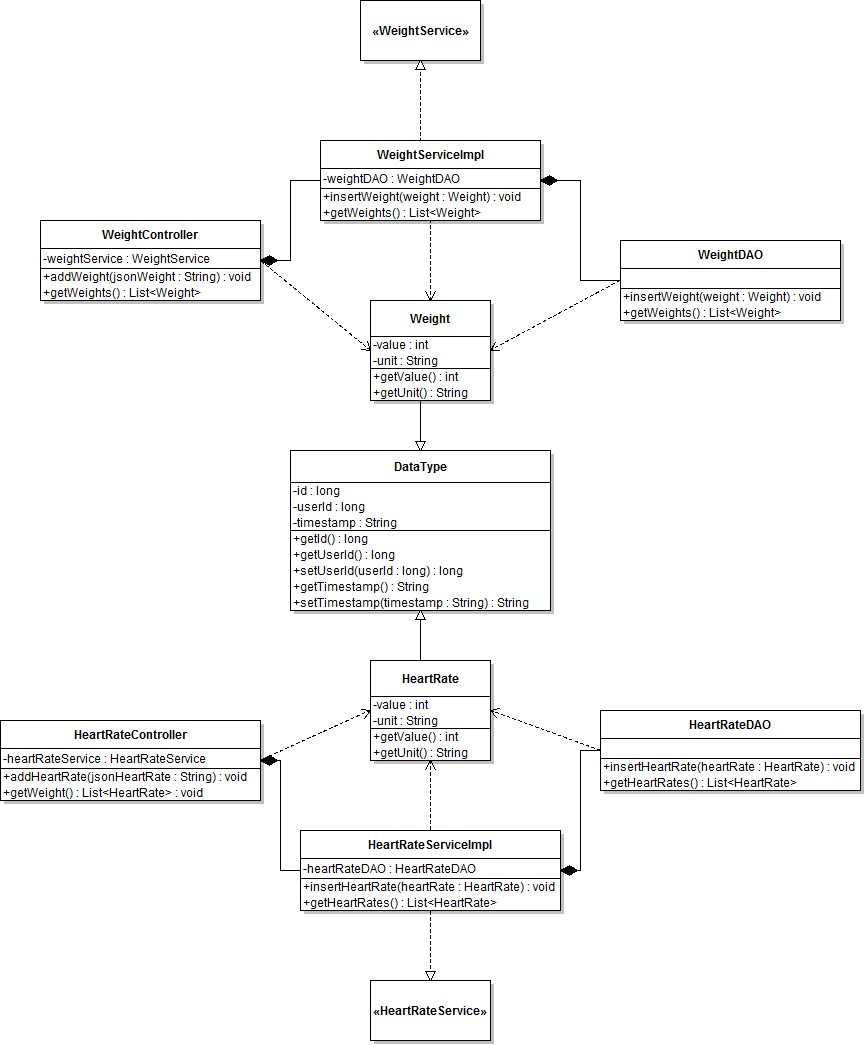
\includegraphics[scale=0.5]{../Figures/NIPEN-class-diagram.png}
\caption{NIPEN class diagram}
\label{figure:nipen-class-diagram}
\end{figure}

We are following a MVC (Model-View-Controller) architectural pattern. 
This pattern is ideal for large-scale, team-based development.
It reduces code complexity and offers great code reuse. 
What this means is that we have divided our application into three main parts: models, views and controllers.

\begin{itemize}

\item Model: A model is a data structure that is used within an application.
In our case the models of our application are: Weight and HeartRate.
This classes are filled with data from the database and are used when sending data to the front-end.
They are also used to store data into our database.

\item View: A view is something that displays the data from the models to the users.
The front-end is the view in our case.
How the front-end works is described in subsection \ref{subsec:front-end}.

\item Controller: The controller is responsible for updating the models that are going to be used in the view.
In our application the controllers are called when a HTTP GET or HTTP POST request is sent to a specific URL.
The controllers work as an interface that connects the applications we have developed with our back-end.

\end{itemize}

\subsection{Data models}
\label{subsec:models}

We decided to represent our data models using JSON.
Although there were other perfectly viable alternatives like XML,
we opted for JSON because it is less verbose and we had previous experiences with it.
Additionally, JSON APIs are used by major networking services which deal with huge amounts of
data like Facebook and Twitter.
%We are using JSON strings when transmitting data to and from the server.
%The representation of the data is inspired from the Human API.
human/api, described in section \ref{section:humanapi}, provided a good starting point for the design of
these models which we have simplified and adapted to our needs.
Both heart rate and weight measurements have \iffalse are represented with\fi the same attributes.
This is due to the fact that their are rather simple measurements which involve nothing more but
a user's ID, a value, a unit, and a timestamp.
%They contain an ID, user ID, timestamp, value and a unit.
%The ID is not needed, when the JSON string is sent, because it is created on the server side.
%Below is a representation of a heart rate JSON string that can be used to store heart rate data on the server:
See below an example of JSON model for heart rate measurements.

\begin{lstlisting}[language=json]
{
	"userId":1,
	"timestamp":"2013-10-27 14:57:39.0",
	"value":75,
	"unit":"bpm"
}
\end{lstlisting}

A weight model looks pretty much the same (see below), but uses another unit.
%The ID of the data is shown when receiving the data from the server:

\begin{lstlisting}[language=json]
{
	"userId":1,
	"timestamp":"2013-10-27 14:57:39.0",
	"value":90,
	"unit":"kg"
}
\end{lstlisting} 

\subsection{Web API}
\label{subsec:api}

NIPEN exposes a JSON based web API to store and retrieve health information.
% which other applications can use to interoperate.
By using a web API, we ensure that the system is accessible to a broad number of users
an from a wide selection of devices. All that is needed is an internet connection.
In fact, the API is exposed to the web via a web server, in this case Apache Tomcat 7.
There were of course a number of alternative web servers we could have used but we sticked
with Tomcat because we had used it before and it provided all needed functionality.
Applications can interact with NIPEN by issuing HTTP GET and POST messages to pre-defined URLs called API endpoints.
Internally, these methods are handled by Spring \textit{Controllers} which implement the logic of the API.
Each API endpoint is associated with a resource and an action to be perfomed on it as shown in table \ref{table:api}.
%What this means is that we are using HTTP methods to request and send data.
%We have two controllers that handle the API calls, concerning the heart rate and weight data, in our system.
%They are called \textit{HeartRateController} and \textit{WeightController}. 
%The \textit{HeartRateController} controls retrieval and storage of heart rate, while 
%the \textit{WeightController} handles weight data.
%These controllers handle two HTTP methods, POST for pushing data and GET for retrieving data.
%When requesting data from our API an HTTP GET request needs to be performed to one of the following URLs:

\begin{table}[h]
\begin{center}
\begin{tabular}{ | l | l | c | c | }
	\hline
	Resource	& URL						& HTTP Method 	& Action \\
	\hline
	Heart rate	& /nipen/api/heart\_rates	& GET			& Read \\
	Weight		& /nipen/api/weights		& GET			& Read \\
	Heart rate	& /nipen/api/heart\_rate	& POST			& Write \\
	Weight		& /nipen/api/weight			& POST			& Write \\
	\hline
\end{tabular}
\end{center}
\caption{API endpoints}
\label{table:api}
\end{table}

When an application makes an HTTP GET request at the URL \verb|/nipen/api/heart_rates| it is returned a JSON
string representing a collection (array) of all heart rate measurements stored in the database.
See below for an example:
\begin{lstlisting}[language=json]
[
	{
		"id":319,
		"userId":1,
		"timestamp":"2013-10-21 07:35:32.0",
		"value":70,
		"unit":"bpm"
	},
	{
		"id":320,
		"userId":1,
		"timestamp":
		"2013-10-22 17:53:09.0",
		"value":66,
		"unit":"bpm"
	}
]
\end{lstlisting}
\label{listing:jsonarray}

Similarly, the application is returned a collection of all weight measurements when making an HTTP GET
request at: \verb|/nipen/api/weights|. Figure \ref{figure:seqhr} shows a sequence diagram for
retrieving heart rates.

\begin{figure}[h]
\centering
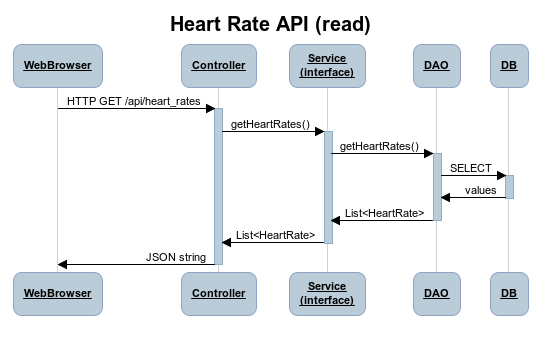
\includegraphics[scale=0.8]{../Figures/seqhr.png}
\caption{Retrieving heart rates from the database}
\label{figure:seqhr}
\end{figure}

When an HTTP POST operation is performed on either \verb|/nipen/api/weight| or \newline
\verb|/nipen/api/heart_rate| then the JSON payload will be translated into a MVC model and
stored into the database. See figure \ref{figure:seqw} for a sequence diagram.

\iffalse
\begin{itemize}
\item $<$server address$>$/nipen/api/human/heart\_rate
\item $<$server address$>$/nipen/api/human/weight
\end{itemize}

With the POST method a JSON string with the specified data type needs to be sent. 
How the controller handles this message is shown in figure \ref{figure:pushing-weight-into-NIPEN}.
The diagram shows an example of how to push a weight value into NIPEN.
The application works the same way when pushing a heart rate value into the system.
When the application receives the JSON string, it first needs to parse it into its respective model class.
After that it is sent to a service class which then sends it to a database handler class.
This class stores the value into the database.
\fi

\begin{figure}[h]
\centering
%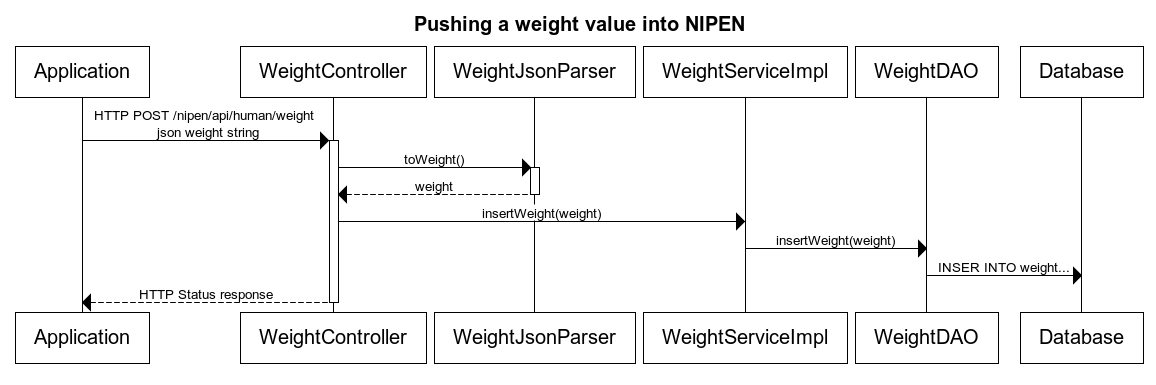
\includegraphics[scale=0.55]{../Figures/pushing-weight-into-NIPEN.png}
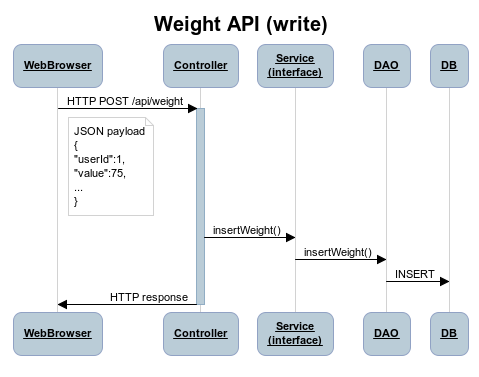
\includegraphics[scale=0.8]{../Figures/seqw.png}
\caption{Pushing a weight value into NIPEN}
\label{figure:seqw}
\end{figure}


\subsection{Database}

In order to implement persistency of health information we are using a MySQL database.
Although there were some alternative database implementations we opted for MySQL
because we were familiar with it and it offered all the features we needed.
%We are using a MySQL database for data storage.
The whole database is very simple and consists of two tables only: one for each supported health measurement.
%one for heart rate and one for weight.
%The heart rate table is shown in figure \ref{figure:heart-rate-database-diagram}
%and the weight table in figure \ref{figure:weight-database-diagram}.
The tables are shown in figure \ref{figure:heart-rate-database-diagram} (heart rate)
and \ref{figure:weight-database-diagram} (weight).
Although the tables are identical, we didn't want to merge them because it would 
have been a bad idea generally, making queries more expensive on large amounts of data.

%As we can see the tables are identical, the only difference is the name.
%The reason we didn't merge this tables is to separate the data, and it is also more efficient.
%It would require more resources to separate the data if they all were in one table.

\begin{figure}[h]
\centering
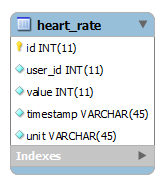
\includegraphics[scale=1.0]{../Figures/heart-rate-database-diagram.png}
\caption{Heart rate database diagram}
\label{figure:heart-rate-database-diagram}
\end{figure}

\begin{figure}[h]
\centering
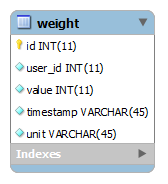
\includegraphics[scale=1.0]{../Figures/weight-database-diagram.png}
\caption{Weight database diagram}
\label{figure:weight-database-diagram}
\end{figure}

Access to the database in NIPEN is implemented by two classes: HeartRateDAO and WeightDAO.
Both provide functionality to read and write entries from/to the respective table in the database.
Having only one access point to the database is generally a good practice because it permits to
identify errors more easily as they can only be in one place.
%We have created separate classes for accessing the database through our server application.
%One for heart rate (HeartRateDAO) and one for weight (WeightDAO).
%This two classes contain a method for inserting and a method for fetching data from the database.
The data that is fetched from the database is ordered by timestamp, so that other applications
don't have to sort it themselves.
%In this way the other parts of the system doesn't need to sort the data afterwards.

%------


\section{Front-end}
\label{subsec:front-end}

The main functionality of the front-end is to visualize the data stored by NIPEN.%the Integration Platform.
This is accomplished by using a regular web-page consisting of HTML, CSS and JavaScript. HTML and CSS are used for structuring and giving a nice design to the web page. With help of JavaScript we are able to make the page dynamic.

\subsection{Design and Visualization}

One of the requirements given by the customer was that the front-end should use helsenorge.no color palette
(see figure \ref{figure:helsenorge-color-palette}).
%That is the front-end should use the colors shown in figure \ref{figure:helsenorge-color-palette}.
The front-end should show how helsenorge.no could represent the data from the integration platform. 
Since it would somehow mimic that page, we though that our web page should look similar to helsenorge.no. 
Hence we didn't only use the colors from the given palette, but tried as well to create a similar structure.

\begin{figure}[h]
\centering
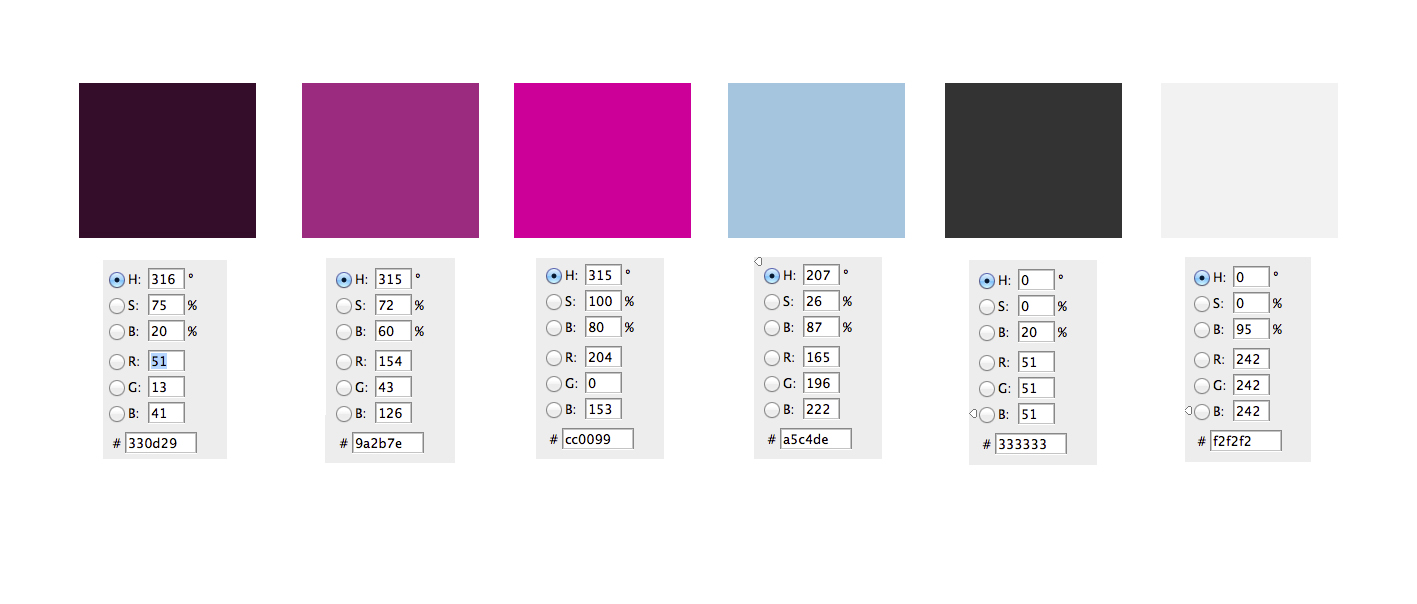
\includegraphics[scale=0.30]{../Figures/helsenorge_pallett.jpg}
\caption{Helsenorge color palette}
\label{figure:helsenorge-color-palette}
\end{figure}

We wanted to keep our front-end simple and user friendly.
%% again shall we mention this in a Limitations section in the conclusion maybe?
%, and since this is only a prototype are we only focusing on one user.
%hence we are only concentrating on how the web page should look like if the user is logged in. 
%Therefore we didn't create any authentication page and thus the user doesn't need to log in. 
%% you say this twice
%The front-end simply consists of one HTML file with some CSS and script files.
Twitter Bootstrap was used as a template to get started with the front-end development.
With help of JavaScript combined with jQuery, were we able to have three web pages in one HTML file. 
The main page \iffalse consists of\fi shows two graphs, one for heart rate and one for weight measurements. 
A visualization of the two latest values measured for each data type is also shown on the left side of the chart.
%Then we have two separate pages for heart rate and for weight.
Charts can also be visualized singularly on separate pages, where they can make use of some more space.
%These pages consists of an enlarged graph of the given data type being viewed.

%%
%This is simply accomplished by hiding the elements that are not used on those pages, and scaling the respective
%graph so it becomes larger.
With help of jQuery it's not a difficult task.
As a bonus jQuery is able to give an animation when hiding, showing and scaling the elements.
This is a nice touch to the web page.

We used a JavaScript library called Chart.js to display health measurements as charts. 
%With help of this library we are able to display the heart rates and weights as bar charts.
This library also has some animations when the graphs are created.
In our application a restriction is given to only display the 10 last measurements in the graphs.
If we have more than that the timestamp of the measurements becomes hard to read.

Figures \ref{figure:frontend-main-page}, \ref{figure:frontend-heart-rate-page} and \ref{figure:frontend-weight-page}
show various pages of the frontend.
%How the web-pages look like is shown in figure \ref{figure:frontend-main-page}, \ref{figure:frontend-heart-rate-page} and \ref{figure:frontend-weight-page}.

%%%% maybe they are too many and too similar?

\begin{figure}[H]
\centering
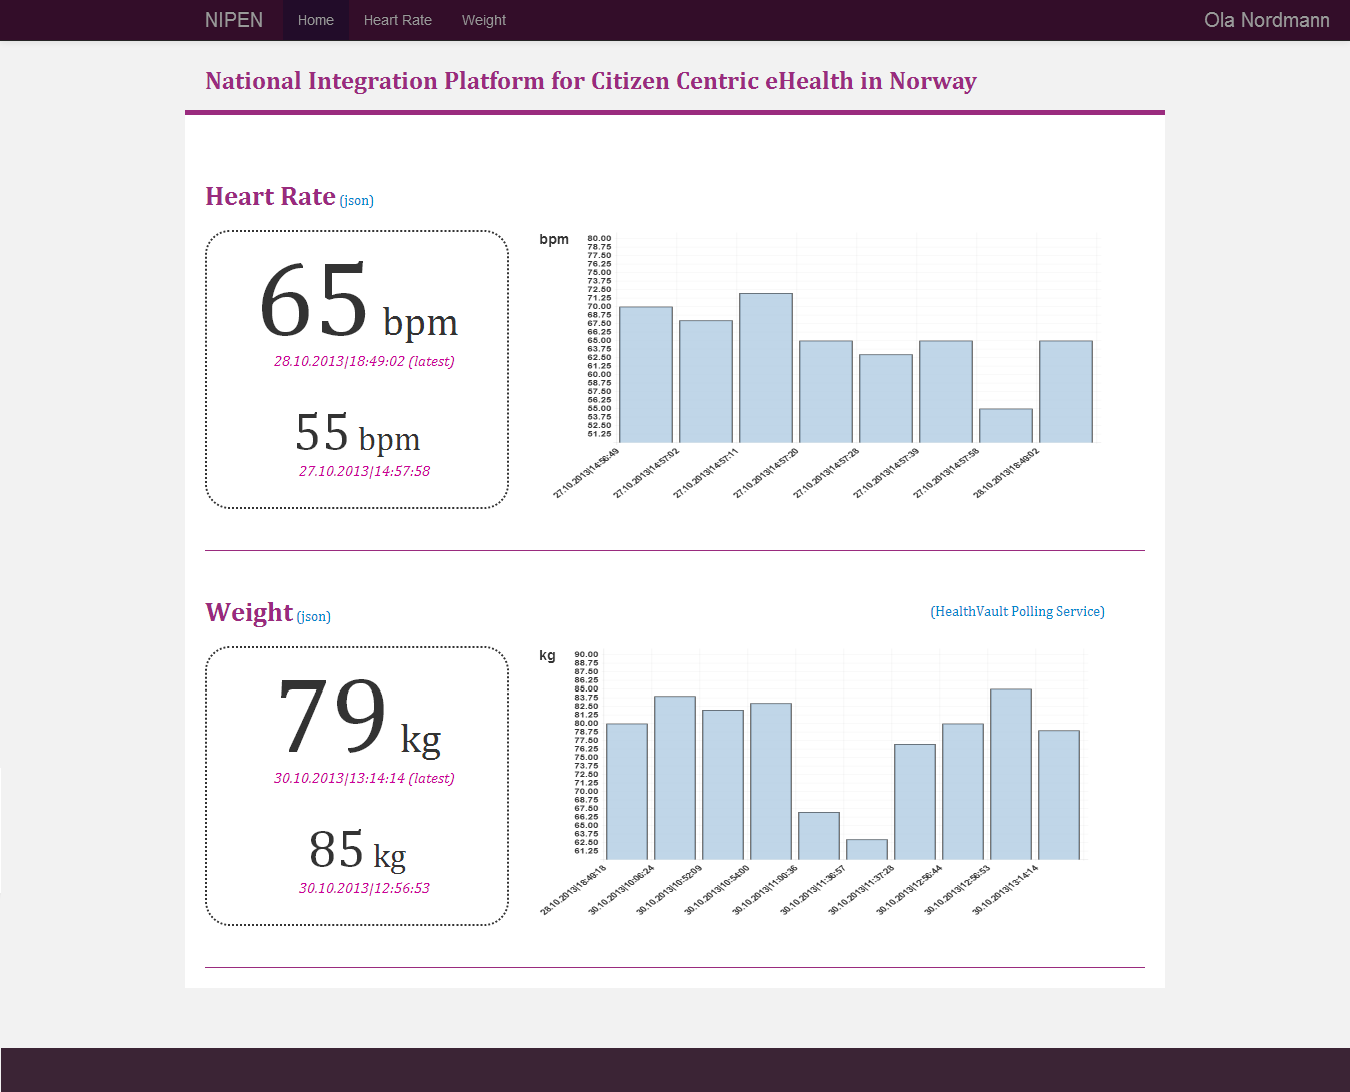
\includegraphics[scale=0.4]{../Figures/frontend-main-page.png}
\caption{Front-end home page}
\label{figure:frontend-main-page}
\end{figure}

\begin{figure}[H]
\centering
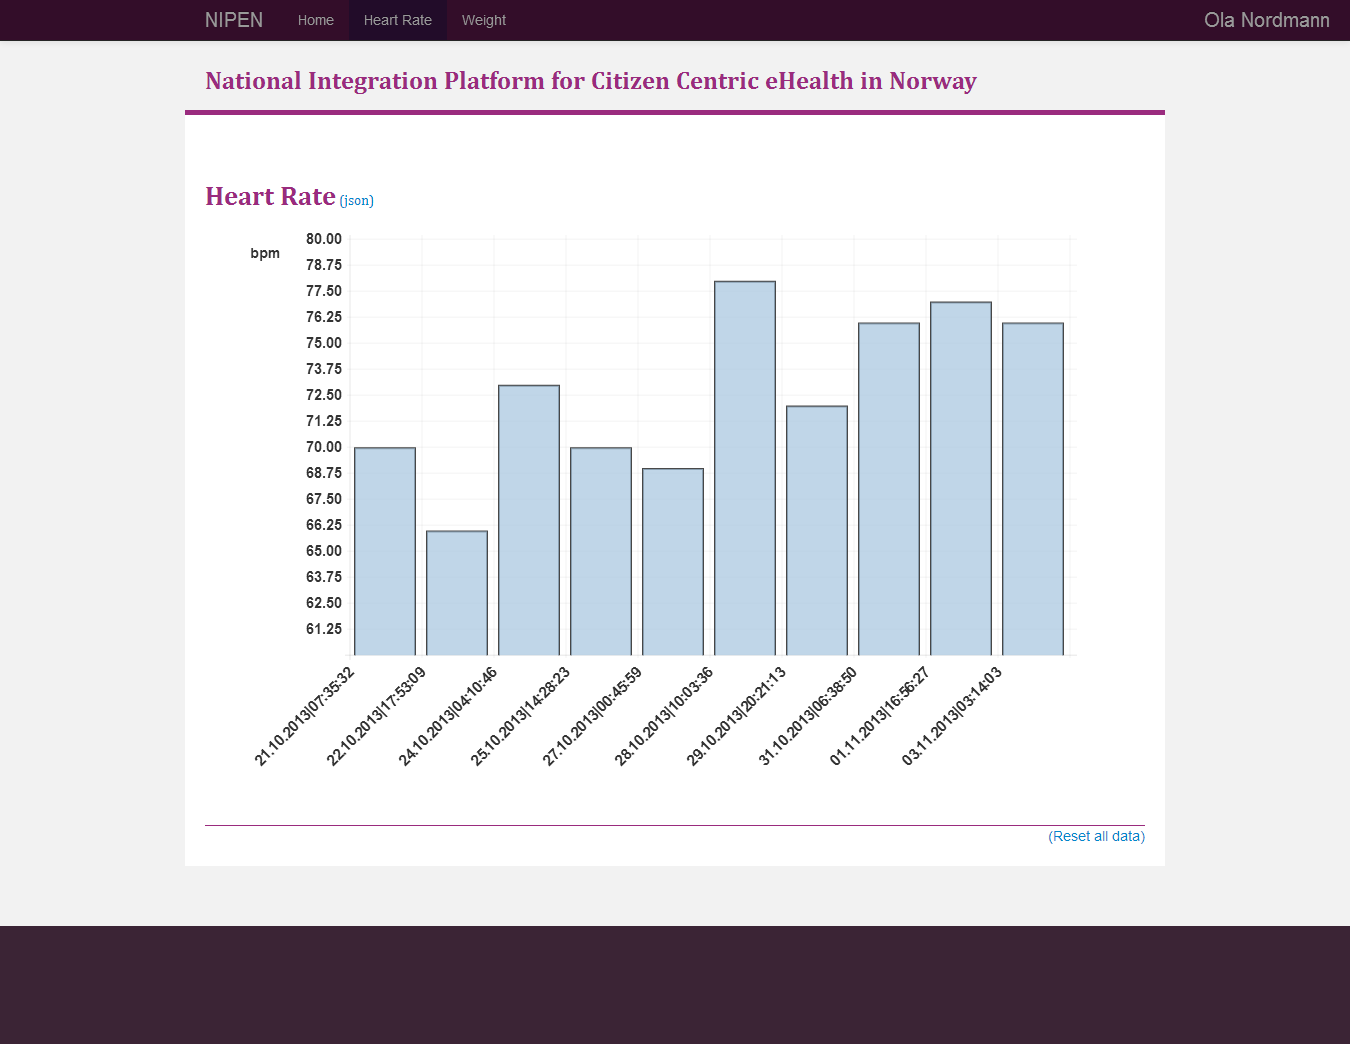
\includegraphics[scale=0.4]{../Figures/frontend-heart-rate-page.png}
\caption{Front-end heart rate page}
\label{figure:frontend-heart-rate-page}
\end{figure}

\begin{figure}[H]
\centering
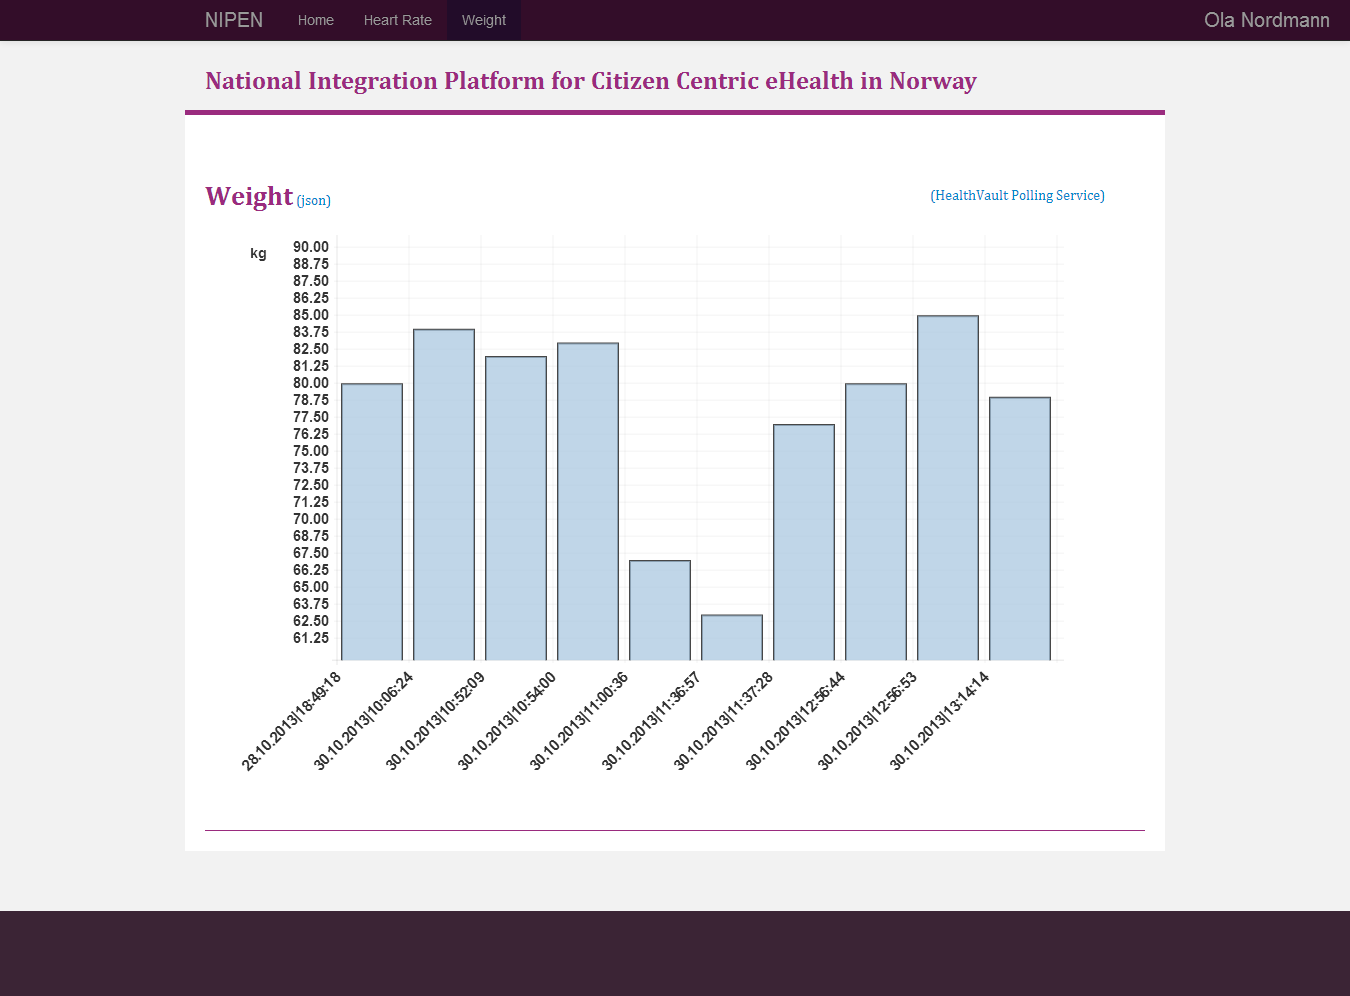
\includegraphics[scale=0.4]{../Figures/frontend-weight-page.png}
\caption{Front-end weight page}
\label{figure:frontend-weight-page}
\end{figure}

\subsection{Retrieving the Data}

To retrieve the data from NIPEN the front-end performs an API call just like any other application.
This is achieved by using AJAX through jQuery. An example \iffalse The structure of the call\fi is given below:
\begin{lstlisting}[language=JavaScript]
$.ajax({
  url: url, // the URL address, e.g.: <server address>/nipen/api/human/weights
  dataType: "json", // the data type of the received data, in this case a JSON string
  success: function(data) {
	// update web page here with the received data
  }
});
\end{lstlisting}

Accessing the JSON data with JavaScript is easy.
%Let's say that the data parameter, of the success function given above, consists of the following JSON array:
Let's say that the data parameter, of the success function given above, consists of the JSON array show precendently 
in subsection \ref{listing:jsonarray}.

\iffalse
\begin{lstlisting}[language=json]
[{
	"id":1,
	"userId":1,
	"timestamp":"2013-10-25 14:57:39.0",
	"value":80,
	"unit":"kg"
},
{
	"id":2,
	"userId":1,
	"timestamp":"2013-10-30 16:40:30.0",
	"value":81,
	"unit":"kg"
}]
\end{lstlisting}
\fi

Then the data can be accessed the following way:
\begin{lstlisting}[language=JavaScript]
data[0].id // returns 1
data[0].userId // returns 1
data[0].timestamp // returns "2013-10-25 14:57:39.0"
data[0].value // returns 80
data[0].unit // returns "kg"

data[1].id // returns 2
data[1].userId // returns 1
data[1].timestamp // returns "2013-10-30 16:40:30.0"
data[1].value // returns 81
data[1].unit // returns "kg"
\end{lstlisting}

This data is used in an update function, that updates all the values that are needed on the web page.
%% not really clear what you mean here.

\subsection{Polling}

We decided to implement polling on our front-end, since we are using AJAX to update the page.
AJAX is asynchronous which means that it can poll data in background without the need of refreshing the page.
Thus we don't need to update the web page when new data is received at NIPEN.
The jQuery AJAX function is polling constantly in the background when the client views the page.
When the front-end detects that new data is received, the JavaScript methods will update the page.
To detect if the data received from NIPEN is new, we compare the timestamp of the latest value on the web page and the data received.
If this value is different, the charts and values on the web page needs to be updated.
This will be done automatically.
Of course, if data is added with a timestamp that contains a date earlier than the latest, then the web page 
will not be updated.
In this scenario the user must manually refresh the web page.

\section{Heart rate application}

The heart rate application is an application for Android mobile devices.
It's purpose is twofold: on one side it demonstrates the praticality of gathering health parameters using mobile phones,
on the other, it shows how easily these can be intregrated with NIPEN. % memorized, stored ?
The application was developed using an open source project called \verb|android-heart-rate-monitor| described
in subsection \ref{subsec:hr} which features an algorithm to measure heart rate using the phone's camera.
%We are using the open source  \cite{AndroidHeartRateMonitor} app as our base to our hart rate application.
Not having to implement such functionality ourselves allowed us to dedicate time to other tasks.
Being only three people on a large project like this, we though that it would be great idea.
%The existing android heart rate monitor app is capable of measuring a users heart rate.
We have extended the application to be able to send measurements to NIPEN.
To do so, the application constructs a valid JSON string representing an heart rate model and then
sends an HTTP POST message to the appropriate API endpoint containing the JSON string as payload.

%% this is mostly okay but too long to be this detailed.
%% i summarized it in a few senteces cutting out some boring details
\iffalse
To construct a valid heart rate JSON string we need user ID, timestamp, value and a unit. 
An ID is not needed because it is constructed at the back-end.
The user ID is a hard coded value, since we are only focusing on one user.
From the android device we are able to get the current time, the heart rate value is calculated through the
app and the unit is BPM (beats per minute).
With this information we are able to construct the JSON string that is needed to push a heart rate value into NIPEN.

To send the JSON string, we need to create an HTTP connection with NIPEN.
We are using the java class \textit{java.net.HttpURLConnection} for this task.
To initialize the URL connection we need to set the request method to POST and the content type to \textit{application/json}.
The URL is set to \textit{http://mhealthdemo03.cloudapp.net/nipen/api/human/heart\_rate}, where \textit{mhealthdemo03.cloudapp.net} is the server location as of this writing.
From the http connection we are able to get an output stream where we write the JSON message.
If we are not getting an exception at this stage, it means that the data was successfully transmitted.
\fi

A simple sequence diagram of how the application works is presented in figure \ref{figure:sending-heart-rate-through-app}.
What we have added to the application is the last part, i.e. from where the users presses the button.

\begin{figure}[h]
\centering
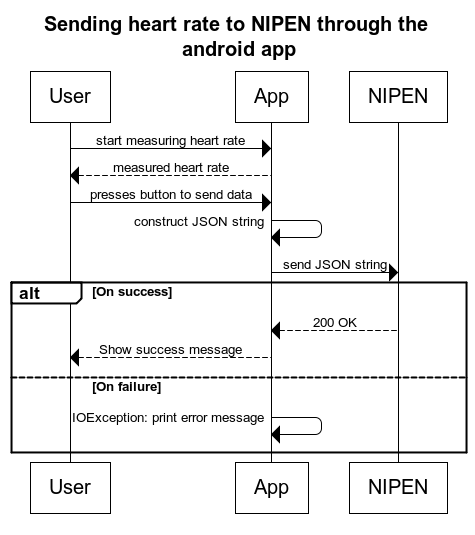
\includegraphics[scale=1.0]{../Figures/sending-heart-rate-through-app.png}
\caption{Sending a heart rate through the android app}
\label{figure:sending-heart-rate-through-app}
\end{figure}

\section{Weight application}

The weight application is an Android app that is able to fetch and push data to and from HealthVault, as well as
it is it capable of pushing data to NIPEN.
We are also using an existing solution as a base for this application, where the features we implemented are
the interactions with NIPEN.
The base we are using for this application is an example from the HealthVault Java SDK \cite{HealthVaultSDK}.
When the SDK is downloaded, it contains a folder named \textit{android}. 
This folder again contains a folder \textit{examples} where the base, we are using, is located.

When the application starts it asks the user to sign in to HealthVault.
If this is the first time the user uses this application he/she is asked to add this application to HealthVault,
after the sign in process.
When the user grants permission to the application, it is allowed to push and fetch data to and from HealthVault.

How the application works (after login) is illustrated in figure \ref{figure:sending-weight-to-healthvault-and-nipen}.
The functionality we implemented is the construction of the JSON string and the sending of the data to NIPEN.
This is developed almost exactly as the heart rate application, and hence is not further explained here.
The only difference is that we are creating a weight measurement instead of a heart rate.

\begin{figure}[h]
\centering
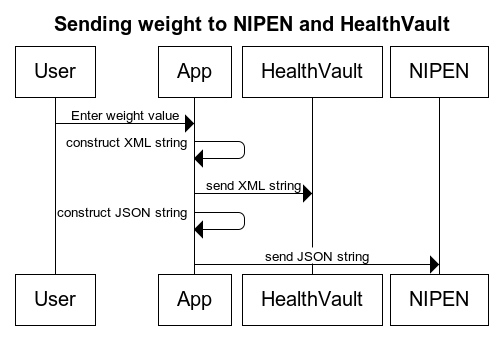
\includegraphics[scale=1.0]{../Figures/sending-weight-to-healthvault-and-nipen.png}
\caption{Sending weight to HealthVault and NIPEN}
\label{figure:sending-weight-to-healthvault-and-nipen}
\end{figure}

This application illustrates that it is possible to connect HealthVault into NIPEN.
If the user adds this application to HealthVault, it has access to all the weight values the user has added to the HealthVault account.
Thus it is possible to thereafter send the values into NIPEN.

\section{HealthVault Integration Service}

The HealthVault integration service is capable of retrieving values from HealthVault and send new values into NIPEN. 
As the weight application, this service uses an example in the HealthVault Java SDK \cite{HealthVaultSDK} as its base.
In the SDK folder it is located inside \textit{java-1.4.2} folder.
The functionality we have implemented into this application is a polling service and the interactions with NIPEN.
We have also made some cosmetic changes to the web pages the example provided.

This application consists of a back-end and a front-end.
What this means is that it consists of a web page and a server application.
The server application is handling the interactions with HealthVault and NIPEN, while the front-end creates a display for the user as well as it processes the users requests.

We have completely changes the look of the front-end of this application.
When the user opens the web page, he/she is asked to login into HealthVault.
The procedure for the login is the same as the weight application.
Figure \ref{figure:webservice-login} shows how the login page looks like.
After the user has signed in, a web page is shown where it is possible to start/stop the polling service.
Is is also possible tof push weight data into HealthVault. 
This is illustrated in figure \ref{figure:webservice-not-polling} and \ref{figure:webservice-polling}.

\begin{figure}[H]
\centering
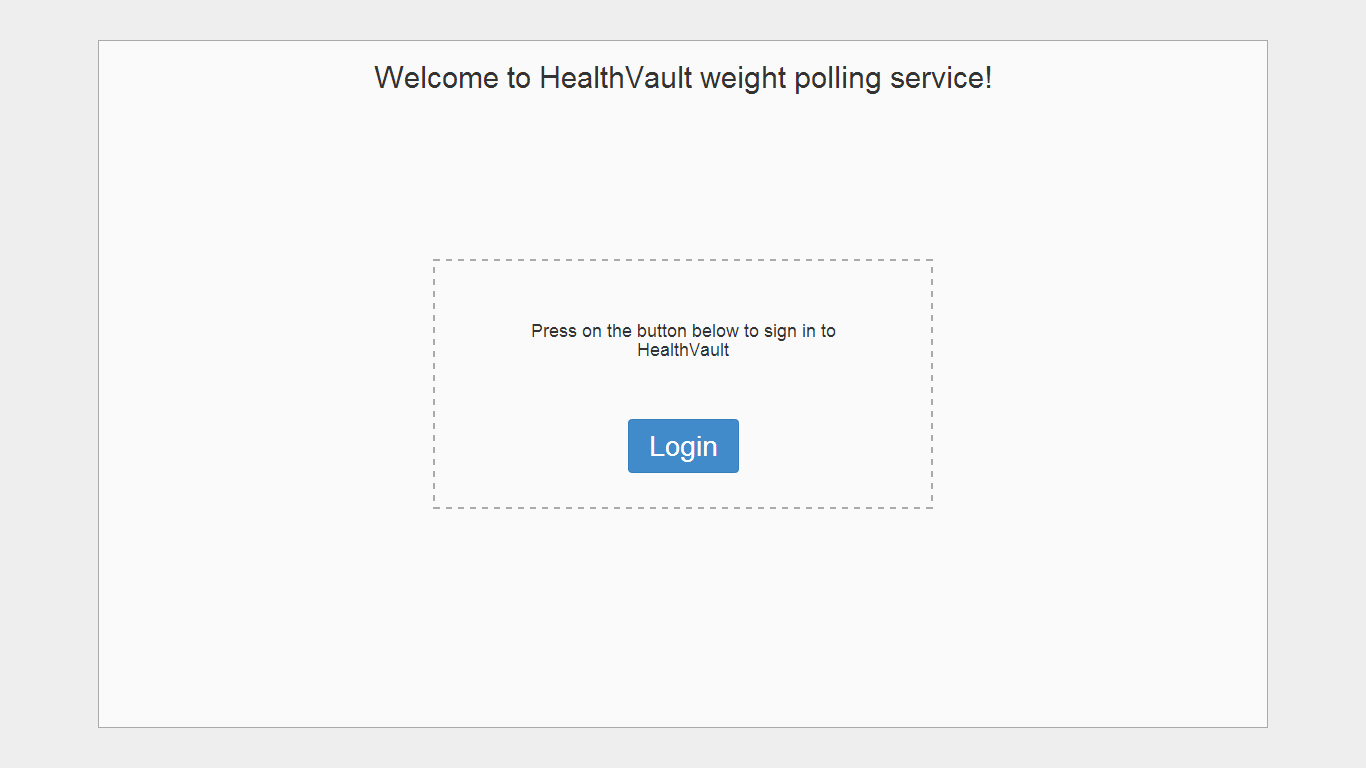
\includegraphics[scale=0.4]{../Figures/webservice-login.png}
\caption{HealthVault Integration Service login page}
\label{figure:webservice-login}
\end{figure}

\begin{figure}[H]
\centering
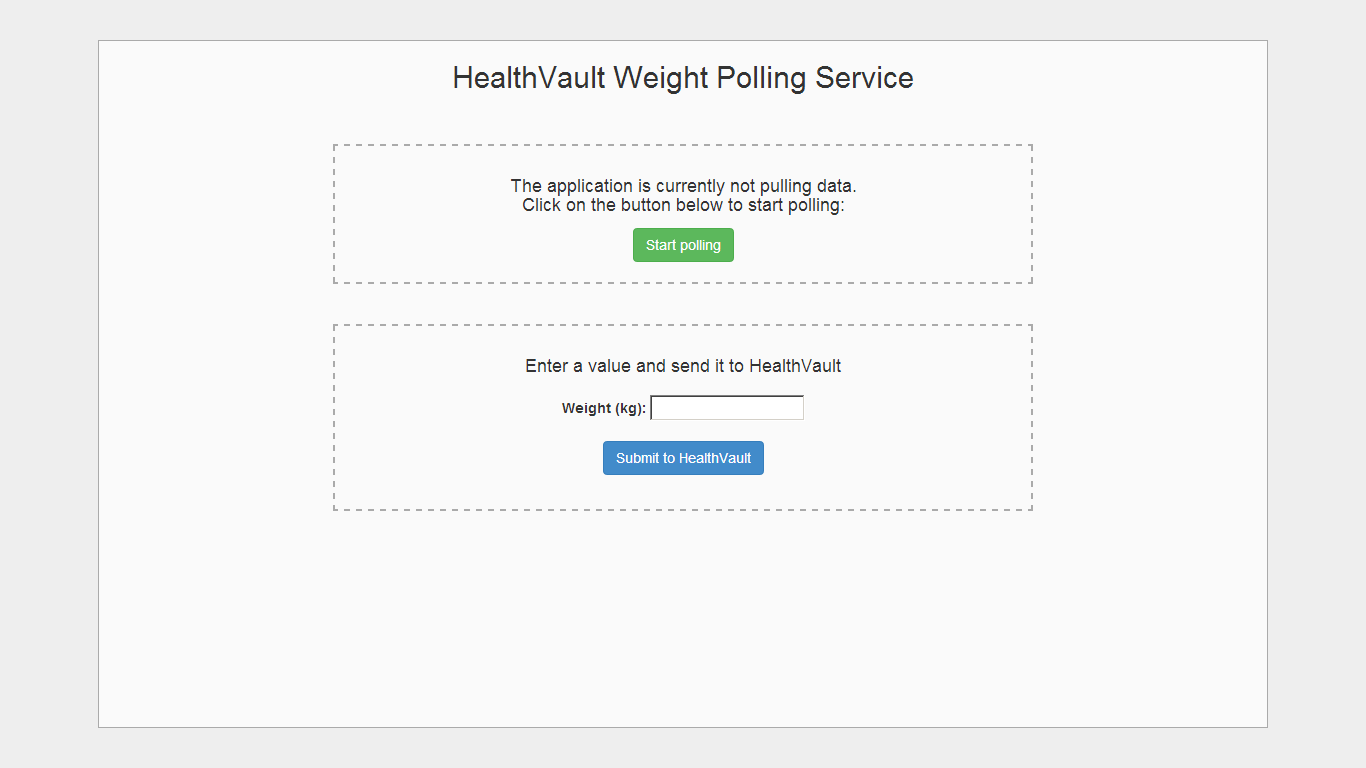
\includegraphics[scale=0.4]{../Figures/webservice-not-polling.png}
\caption{HealthVault Integration Service not polling page}
\label{figure:webservice-not-polling}
\end{figure}

\begin{figure}[H]
\centering
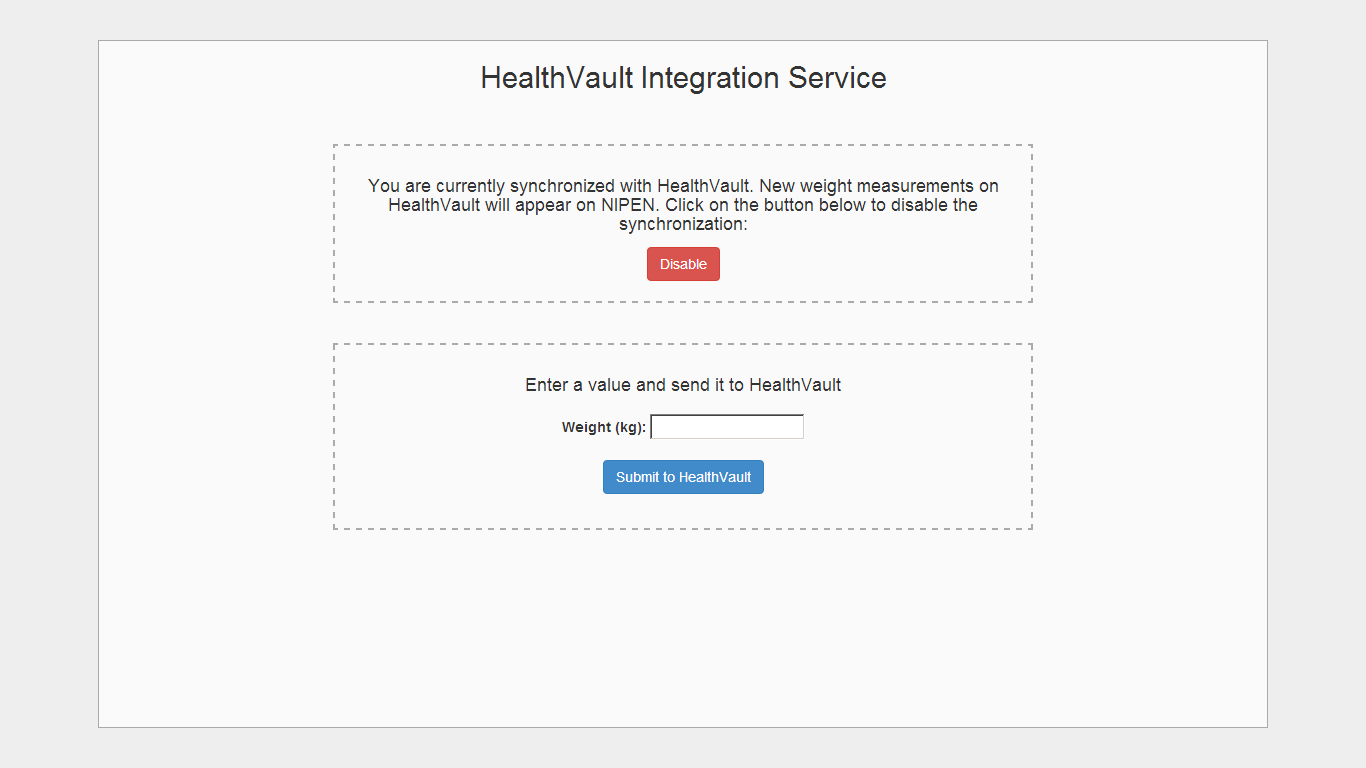
\includegraphics[scale=0.4]{../Figures/webservice-polling.png}
\caption{HealthVault Integration Service polling page}
\label{figure:webservice-polling}
\end{figure}

When the user has signed in to HealthVault through the application, an authentication token is sent from HealthVault.
This token is received and stored in the web service.
What this token does is that it allows the application to fetch weight data from HealthVault.
After the sign in the user can start the polling service.
When the user requests the application to start polling, a thread is created on the back-end.
This thread starts fetching data from HealthVault on a regular basis.
Every time the application receives data it waits 1 second and then fetches again.
This is repeated until the user stops the polling service.

When the polling starts the application stores the first timestamp, of the last weight measurement, received from HealthVault.
After that, for each poll the application compares this timestamp with the timestamp received from HealthVault.
A new value will be added to HealthVault if the timestamps are not equal.
If a new value has been detected, the application creates and sends a JSON string to NIPEN in the same way as the heart rate and weight application.
The polling service is illustrated in figure \ref{figure:weight-polling-service}.

\begin{figure}[h]
\centering
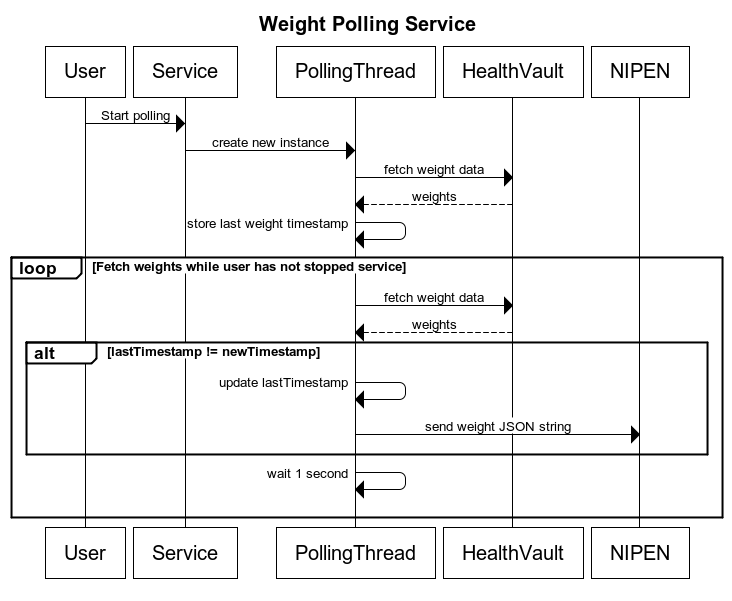
\includegraphics[scale=0.8]{../Figures/weight-polling-service.png}
\caption{HealthVault Integration Service sequence diagram}
\label{figure:weight-polling-service}
\end{figure}

\section{Rationale}

We had to make multiple important choices in technologies before starting our development process.
Why we choose the different solutions is discussed in this section.

\subsection{Modular architecture}
Our choice of a modular architecture, where components could be developed separately,
allowed us to implement functionality little by little and have demonstrable
system ready at any time with the use of mockup components if needed.
This has let us avoid delivering our product all at once, reducing the risk
of last-minute implementation problems to affect the outcome of the project.
Additionally, it enabled us to modify the overall system architecture with ease
if necessary, adding or removing application prototypes.

%Having used a approach were the product was delivered
\iffalse
Duo to the lack of resources and time constraints we needed to apply a sort of evolutionary architecture during our development process.
In this way we could start of with a simple application and add functionalities to it later on.
We started of by implementing the functionalities regarding the heart rates. 
Later on we added support for weights.
Since an architectural driver was that the system needed to have a degree of interoperability, we were able to develop our front-end, heart rate application and both of our weight applications separately.
This was accomplished by defining the interfaces, i.e. the data models that are being sent between NIPEN and the applications, early on.
Because of this it was easy to add applications to the system at a later point.
\fi

\subsection{Communication}

Since we are making an integration platform we needed to decide in what way this system should interact with other applications.
Communication can be performed with a RESTful service or SOAP.
However, from the functional requirements it was already specified that the system needed to receive and forwards data in form of JSON strings.
SOAP mainly uses XML and hence a RESTful service was a better choice.
This type of service doesn't require any specific format of data that is sent or received, whereas SOAP has some strict rules.
With REST we have the possibility to send raw JSON strings between our applications.
JSON strings are also easily handled by JavaScript.
Although we are not implementing all of the methods REST supports we are covering the most important ones, this includes GET and POST for receiving and sending data respectively.

\subsection{Visualization of data}

The data gathered by the integration platform had to be shown to users in an intuitive way.

\iffalse
The functional requirements claimed that we needed a front-end for visualizing the data that NIPEN had gathered.
A non-functional requirement said that it also needed to have a degree of accessibility.
\fi

We figured that a desktop application would have restricted the accessibility
of the system in a number of ways. Firstly, the user would have had to download
and install the application. This could be a task that some user are unable to perform.
Additionally, we would have had to provide support for different platforms such as
Windows, Mac OSX\ldots.
Hence, we though that a web page would be the best way to let users visualize
the data acquired by the system. It permitted us to code the functionality
once and make it available everywhere.

%Users would then need to download the application in order to view the data.
%We would also need to take into consideration what platforms the application should support.
%Hence it was a much easier solution to use a web page.

The front-end also needed to visualize this data in form of charts.
Duo to time requirements and lack of resources we decided to use a open source library for this task.
Hence we chose Chart.js for this task.
To make it easier for us to develop the front-end we also used jQuery and Bootstrap.
jQuery was a good choice since we already had some experience with this framework.

\subsection{Server technologies}

The customer gave us a choice between a Windows Server and an Ubuntu Server.
Since some of us already were familiar with Linux we chose the Ubuntu Server.
We decided to develop the server application in Java with Spring as a framework for helping us to implement the API endpoints.
This is because all of us already were familiar with Java, and some of us also had some experience with Spring.

\subsection{Mobile applications}

For the heart rate application we needed a programmable device with an internet connection, a camera and a screen.
The weight application needed mainly a screen and an internet connection.
Since all of us already had an android mobile we choose to develop our heart rate and weight application for these devices.

\subsection{Existing solutions}

We are using mainly existing solutions for the application that are sending values into NIPEN.
This is because of the business constraints covered in subsection \ref{subsec:business-constraints}.
The reason we chose the selected applications as our base is because they already contained all the main functionality that were needed in our situation.
The base for the heart rate application was able to measure heart rates.
It was also developed for Android using Java and Android SDK.
We were already familiar with these technologies, and hence we thought that this open source application would be a good starting point for our heart rate application.
The foundation of the weight application and the HealthVault integration service had already implemented communication with HealthVault.
In addition it was programmed in Java which we already were familiar with.